\documentclass[12pt]{article}
\usepackage{tikz}
\usepackage{circuitikz}
\usepackage{amsmath}
\usepackage{amssymb}
\usepackage{graphicx}
\usepackage{float}
\usepackage{geometry}
\usepackage{pgfplots}
\usepackage{color}
\usepackage{xcolor}

\geometry{a4paper, margin=1in}
\pgfplotsset{compat=1.18}

\begin{document}
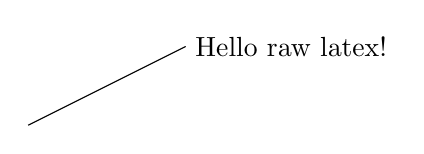
\begin{tikzpicture}
  \draw (0,0) -- (2,1) node[right] {Hello raw latex!};
\end{tikzpicture}
\end{document}
